\chapter{Implementation}
\label{chap:impl}
The implementation of
the robot memory is separated according to the layered
architecture. \refsec{sec:back-end} presents the implementation of the
back-end containing the MongoDB databases and \refsec{sec:impl-memory}
presents the implementation of the robot memory with the operations-,
trigger-, and computable manager. Both application layers are covered
in \refsec{sec:impl-planner}. We conclude with the description of the
evaluation scenarios and how they were implemented in
\refsec{sec:applicationscenarios}.

\section{MongoDB Back-End}
\label{sec:back-end}
The back-end of the robot memory is based on MongoDB databases. It
acts as storage of the robot memory and executes insert, query,
update, and delete operations. The representation of stored information
utilizes the document structure of MongoDB with key-value pairs and
nested sub-documents. This allows a flexible storage of
information pieces in the structure that is induced by the application
and can be expanded by meta information from the robot memory.

\begin{wrapfigure}{r}{0.47\textwidth}
  \vspace{-0.8cm}
\begin{lstlisting}[style=SmallJSON,
  caption={Representation of a knowledge item in the back-end},
  label=lst:backend,
  framexleftmargin=1pt, xleftmargin=0pt,
 morekeywords={}, numbers=none]
 {
   _robmem_info:
   {
     persistent: true,
     decay_time: ISODate(
       "2016-05-19T 23:50:00.000Z")
   },
   type: "object info",
   name: "milk_1",
   position: {x:2.5, y:1.0, z:0.0},
   storage_place: "refrigerator"
 }
\end{lstlisting}
\vspace{-8mm}
\end{wrapfigure}
An example document stored in the back-end is shown in
\reflst{lst:backend}. It contains knowledge about a bottle of milk, as needed
by a planner told to bring it, with additional information where it
should be stored later. Additionally the document contains meta
information needed by the robot memory, e.g., if the document should be
stored persistently or removed at restart and when it should be
dropped because its use-time has expired. How these documents are
parsed, serialized, stored, and queried again is handled by
MongoDB. To connect to MongoDB from the robot memory, we use the
\texttt{mongodb} plugin in Fawkes. It was developed for the
implementation of the Generic Robot Database~\cite{RoboDB} and
utilizes the C++ driver of MongoDB. We also extended this plugin,
e.g. to properly connect to a distributed replica set.

As the architecture in \reffig{fig:arch} shows, the MongoDB backend
contains a local and a shared part. Each part is operated by a
separate \texttt{mongod} instance, which is the daemon process of the
MongoDB system. It manages data access, handles data requests, and
performs background management operations. Each \texttt{mongod}
instance is accessible over its unique TCP port and can contain multiple
databases. The databases of the robot memory that are only locally
relevant are managed by the local \texttt{mongod} instance. The shared
\texttt{mongod} instance manages the distribution of shared databases
in a multi-robot system. Thus we configured it to be part of replica
set as already described in \refsec{sec:mongodb}. This ensures the
efficient distribution of the databases and handles important
distribution issues, such as Primary election, consistency, and
synchronization. The
robot memory needs multiple connections to both \texttt{mongod}
instances because single connections, as provided by the C++ driver,
are not thread safe. Thus we use the connection manager of the
\texttt{mongodb} Fawkes plugin to create two connections each for
operations, computables, and triggers. After some experiments with sharding, we decided
against using it to ensure that at least one robot has write access to
the full robot memory. Based on our experience of WiFi issues in the RCLL,
where the network was unusable for several seconds, it can be a
problem that every robot could have to wait until a Primary for a shard of
the world model is reachable.
Furthermore we expect that the classical motivation for sharding,
namely a bottleneck in processing power for updates, is not given.

The MongoDB back-end also contains the operations log (Oplog), a
separate capped collection containing the list of changes to the
database with a timestamp. The Oplog is accessed by the robot memory
to analyze database changes for triggers. However, the Oplog is only
created for replicated database, because its original purpose is
logging changes to propagate them to other instances in the Replica
Set. Thus we also have to configure the local \texttt{mongod} instance
as Replica Set, but this set only contains itself because its
databases are only locally relevant.

Because the robot memory requires a special configuration of the
MongoDB daemons, we also implemented an automated setup of the
back-end. This setup starts the \texttt{mongod} processes as
sub-processes of Fawkes if they are not already running. Each process
needs to be configured, most importantly, with the Replica Set name,
the database path, where the databases are persistently stored on the
hard-drive, and the Oplog size. After the start-up, the \texttt{mongod}
instances need to be initialized, when they are started for the first
time. Thus the automated setup sends commands for initialization of
the Replica Set with information about the members of the
set. Furthermore, commands for the query evaluation are sent, to allow
query evaluation on Secondaries. When Fawkes is terminated, also the
MongoDB sub-processes are finalized again.

\section{Robot Memory}
\label{sec:impl-memory}
The robot memory middle-layer implements most functions of the robot
memory that exceed a typical database. Because this is a central and
large part of this thesis, we split the implementation into the query
language in \refsec{sec:impl-query-language}, the operation manager in
\refsec{sec:impl-opmanager}, computables in
\refsec{sec:impl-computables}, triggers in \refsec{sec:impl-triggers},
and unit-tests in \refsec{sec:impl-unittests}. The robot memory layer
can be accessed in Fawkes through the \texttt{RobotMemoryAspect} and
through sending messages to the blackboard interface of the robot
memory. Both the aspect and the interface are provided by the
\texttt{robot-memory} plugin.

\subsection{Query Language}
\label{sec:impl-query-language}
A central question is which query language should be used between
applications and the robot memory because this determines the
expressiveness and has a large impact on the performance. We choose to
use the query language of MongoDB as it is already used between the
robot memory and the back-end. This has the following advantages compared to
using other query languages, such as SQL, SPARQL,
XQuery~\cite{query-languages}, and JSONiq~\cite{jsoniq}:  For the
applications using the robot memory, the query language of MongoDB is
a good choice because it is an intuitive query language and has been
proven as efficient for usual and well designed queries~\cite{RoboDB}. It is also
highly expressive when using additional JavaScript functions or the
MapReduce paradigm~\cite{mongodb}.
\todo[inline]{example expressive query?} For the robot memory, it
requires no translation before applying queries to the
database. Furthermore it allows extending and modifying queries
because queries are structured as documents with key-value fields and
can be nested or executed in sequence. Another advantage of the
MongoDB query language is that it can easily be parsed, e.g., from a
string by using the MongoDB C++ driver. The resulting object can be
analyzed and modified for example to add key-value pairs or to check
if computables are queried.

\subsection{Operation Manager}
\label{sec:impl-opmanager}
The MongoDB query language provides the basis for the operation
manager, which receives insert, query, update, and deletion
requests. Received requests are analyzed using the MongoDB C++ driver
and modified before being applied to the back-end. This way, the
operation manager can add meta information of the robot memory to
documents and queries, and the computable manager can base its
decision if computables need to be executed on the contents of a
query.

The basic operations on the robot memory are insertions, queries,
updates, and deletions. For all four, the operation specifies on which
collection in which database the operation should be performed. The
collection string contains both separated by a dot,
e.g., \texttt{'robmem.worldmodel'} for the worldmodel collection in
the robmem database. Using
the configurable list of shared databases, the collection string also
specifies whether the operation should be performed on the local or
shared \texttt{mongod} instance. Because connections to MongoDB
are not thread safe, the operation manager has to guarantee the
mutual exclusion of connection usage. Furthermore, the operation
manager handles exceptions caused by operations, e.g. when a query can
not be parsed or an object contains invalid fields.

\begin{wrapfigure}{r}{0.4\textwidth}
  \vspace{-0.4cm}
\begin{lstlisting}[style=SmallCpp,
  caption={Inserting a document about a red cup in C++},
  label=lst:impl-insert,
  framexleftmargin=5pt, xleftmargin=0pt,
 morekeywords={}, numbers=none]
mongo::BSONObjBuilder b;
b.append("object", "cup");
b.append("color", "red");
b.append("clean", false);
b.append("pose",
  fromjson("{x:0,y:1}"));
robot_memory->insert(
  "memory.dishes", b.obj());
\end{lstlisting}
\vspace{-8mm}
\end{wrapfigure}
An \textbf{insertion} operation also specifies the document that
should be inserted. An example insertion of a document in C++ is
shown in \reflst{lst:impl-insert}. The object is built by adding
key-value pairs. The \texttt{position} field holds a sub-document
constructed from a JSON string. Before performing the insertion on the database,
the operation manager can add meta information of the robot memory,
for example the insertion time if the collection is configured to be a
short time memory. The meta information is contained in a sub-document
under the \texttt{\_robmem\_info} key, as shown in
\reflst{lst:backend}.

\begin{wrapfigure}{r}{0.5\textwidth}
  \vspace{-0.4cm}
\begin{lstlisting}[style=SmallCpp,
  caption={Query for printing all cup colors},
  label=lst:impl-query,
  framexleftmargin=5pt, xleftmargin=0pt,
 morekeywords={}, numbers=none]
mongo::BSONObjBuilder q;
q.append("object", "cup");
QResCursor res = robot_memory->query(
  "memory.dishes", q.obj());
while(res->more())
{
  BSONObj cup = res->next();
  std::string color = 
    cup.getField("color").String();
  printf("There is a %s cup.",
    color.c_str());
}
\end{lstlisting}
\vspace{-8mm}
\end{wrapfigure}
For \textbf{queries}, the operation also specifies the query
itself. \reflst{lst:impl-query}
shows how a query can be executed, how to iterate over returned
documents, and how to access their key-value pairs.
The operation manager analyzes the query and modifies it similar
to how it modifies documents. It adds a filter and a read
preference. The filter hides meta information of the robot memory from
the application. The read preference specifies that the query should
be executed closest available of a replica set. This should always be
the local one because it has the lowest latency and thus leads to a
faster query times than performing queries on remote replica set
members. Furthermore the query is passed to the computation manager to
check if a computable has to be executed.

\begin{wrapfigure}{r}{0.5\textwidth}
  \vspace{-0.4cm}
\begin{lstlisting}[style=SmallCpp,
  caption={Update operation to mark one cup in an area as clean},
  label=lst:impl-update,
  framexleftmargin=5pt, xleftmargin=0pt,
 morekeywords={}, numbers=none]
mongo::BSONObjBuilder query;
query << "object" << "cup"
  << "pose.x" << fromjson("{$gt:0}");
mongo::BSONObjBuilder update;
update << "$set" << fromjson(
                    "{clean:true}"));
robot_memory->update("memory.dishes",
  query.obj(), update.obj());
\end{lstlisting}%$
\vspace{-8mm}
\end{wrapfigure}
\textbf{Update} operations contain a query specifying which documents
should be updated and a document containing the changes that should be
applied. An example update operation is shown in
\reflst{lst:impl-update}. It uses shift operators to fill documents
with key-value pairs and the greater than operator \texttt{\$gt}.
By default the first matching document in the specified
collection is replaced by the update document. It is possible to
modify this behavior with additional options. There are options for
perform the update on all matching documents and for inserting the
document even if no document in the collection matches the query
(called \emph{upsert}). To keep key-value pairs in the original
document, the update document needs to contain updated values a
\texttt{\$set} sub-document. In contrast to
query operations, updates do not lead to the execution of computables
because the updated information would be lost shortly after when the computable
exceeds its caching time. However, it is still possible to update
already computed documents because they are handled as regular
documents during the caching time.

\begin{wrapfigure}{r}{0.45\textwidth}
  \vspace{-0.4cm}
\begin{lstlisting}[style=SmallCpp,
  caption={Deletion of all black cups},
  label=lst:impl-delete,
  framexleftmargin=5pt, xleftmargin=0pt,
 morekeywords={}, numbers=none]
mongo::BSONObjBuilder query;
query << "object" << "cup"
  << "color" << "black";
robot_memory->remove(
  "memory.dishes",query.obj());
\end{lstlisting}
\vspace{-8mm}
\end{wrapfigure}
\textbf{Deletion} operations have an attached query specifying which
documents should be removed. \reflst{lst:impl-delete} shows a delete
operation. In contrast to updates, deletions are performed on all
documents matching a query by default.  The operation manager does not
need to perform special modifications of this query.

Additionally to these basic operations, the operation manager can also
export the content of a collection to a file (called \emph{dump}). It
can also import a collection from a file in an operation called
\emph{restore}. These operations can be used to save and load a world
model that is contained in a collection. For example in the RCLL, this
allows setting the world model in a prepared state to test the
behavior of the agent in that state. The dump and restore operations
are implemented by calling the \texttt{mongodump} and
\texttt{mongorestore} command line tools of MongoDB with appropriate
parameters.

\subsection{Computables}
\label{sec:impl-computables}
Computables allow the computation of documents on demand, that is when
a query operation asks for a document that can be provided by the
computable. The computable manager is the entity used for registering
and unregistering computables as well as for checking which
computables should be executed for a query.\\
\begin{listing}
\refstepcounter{listing}
\addtocounter{lstlisting}{1}
\noindent
\begin{minipage}[b]{.30\textwidth}
\begin{lstlisting}[style=SmallJSON,
  %caption={Computable Query},
  %label=lst:comp-def,
  framexleftmargin=5pt, xleftmargin=0pt,
 morekeywords={}, numbers=none]
{
  compute: "sum",
  x: {$exists:true},
  y: {$exists:true}
}
\end{lstlisting}
\captionof{sublisting}{Query defining the computable specification}
\end{minipage}%
\hfill
\begin{minipage}[b]{.25\textwidth}
\begin{lstlisting}[style=SmallJSON,
  %caption={Query requirering computable},
  %label=lst:comp-query,
  framexleftmargin=5pt, xleftmargin=0pt,
 morekeywords={}, numbers=none]
{
  compute: "sum",
  x: 15,
  y: 4
}
\end{lstlisting}
\captionof{sublisting}{Query requiring the computable}
\end{minipage}%
\hfill
\begin{minipage}[b]{.25\textwidth}
\begin{lstlisting}[style=SmallJSON,
  %caption={Computed document},
  %label=lst:comp-res,
  framexleftmargin=5pt, xleftmargin=0pt,
 morekeywords={}, numbers=none]
{
  compute: "sum",
  x: 15,
  y: 4,
  sum: 19
}
\end{lstlisting}
  \vspace{-0.3cm}
\captionof{sublisting}{Resulting document}
  \vspace{0.3cm}
\end{minipage}%
\caption{Queries and documents involved in a computable for addition}
\label{lst:comp}
\end{listing}
\begin{wrapfigure}{r}{0.49\textwidth}
  \vspace{-0.8cm}
\begin{lstlisting}[style=SmallCpp,
  caption={Function of a computable},
  label=lst:comp-func,
  framexleftmargin=5pt, xleftmargin=0pt,
 morekeywords={}, numbers=none]
std::list<mongo::BSONObj>
compute_sum(mongo::BSONObj query,
            std::string collection)
{
  int x = query.getField("x").Int();
  int y = query.getField("y").Int();
  mongo::BSONObjBuilder b;
  b << "compute" << "sum"
    << "x" << x << "y" << y
    << "sum" << x + y;
  return {b.obj()};
}
\end{lstlisting}
\vspace{-8mm}
\end{wrapfigure}
\reflst{lst:comp} and \reflst{lst:comp-func} show how queries,
documents, and functions are involved in a computable by an addition example.
When some component registers a computable
on a collection, it needs to give a reference to the function
performing the actual computation and a definition which documents can
be provided by the computable. This definition is specified by the
\emph{computable spec}, as shown in \reflst{lst:comp}a. Whenever the
robot memory has to answer a query, for example \reflst{lst:comp}b, that is
matched by the computable spec, the computable is executed. The
referenced function for the addition computable is shown in
\reflst{lst:comp-func} and yields a list of computed documents that,
in this example, only contains the result shown in
\reflst{lst:comp}c. The result contains the \texttt{compute},
\texttt{x}, and \texttt{y}, fields because it needs to be matched
later by the original query in \reflst{lst:comp}b.

The computable manager checks whether queries passed to it can be
answered by registered computables. Because the MongoDB C++ driver
supports no unification or matching method outside the database, we
perform the matching inside the database. Firstly the robot memory query is inserted
as document in a separate and empty collection. Secondly the
computable spec is executed as query on that collection to check if the robot memory query
is matched by the computable spec. Thus when the computable spec
returns the robot memory query as result, the function of the computable is called. This function
(\reflst{lst:comp-func}) takes the query causing the computation
(\reflst{lst:comp}b) and the collection as parameters. Thus it can use
values in the query (\texttt{x} and \texttt{y}) to determine what
should be computed. The function then computes a list of resulting
documents (list containing \reflst{lst:comp}c) and returns it to the
computable manager. By defining the computable spec appropriately,
i.e., with \texttt{\$exists}, it is ensured that all values required
by the function are provided by the query. It is also possible have
optional arguments. When optional arguments are not given, a
computable could create documents for all possible values. For example a computable for
blackboard interfaces in Fawkes, could returns documents for all interface
ids of a type, when no interface id is given in the query.

After a computable returned the list of computed documents, the
computable manager inserts these documents in the specified collection
of the robot memory. Finally, the operation manager evaluates the
original query as usual on the collection. The query can return computed
documents as well as persistently stored documents. Thus the computed
information is embedded in the already existing information. Another
advantage of evaluating the original query on the collection, is that
the query can have more key-value fields than required by the
computable, for example to filter computed documents or add
aggregation functions.

To lower the computational effort of computables, we implemented
caching of computed documents. Whenever a query is identical to a
query that caused computation in the caching time before, the no
computables are executed for it. Computed documents remain in the
robot memory during this caching time. This is implemented by adding
the expiration time of computed documents to their meta information
and periodically removing documents with passed expiration time.
A typical caching time could be the loop time of Fawkes.

Computables can depend on the current content of the robot memory, by
using the robot memory themselves in their function. This can be used
for hybrid reasoning by transform documents already contained in the
robot memory into other representations. To allow computables to
depend on the result of other computables, there is a
prioritization. The computable manager uses this prioritization to
determine the order in which computables are checked.

The \texttt{robot-memory} plugin in Fawkes provides two basic
computables. One provides access to the blackboard by computing
documents containing the fields of blackboard interfaces with matching
types and ids. The other transforms documents describing 3D positions
into other frames by using the transform aspect of Fawkes. All other
computables have to be provided by other plugins.
\todo[inline]{example BB computable or TF computable}

\subsection{Triggers}
\label{sec:impl-triggers}
Triggers notify components about changes in the database, for example
to keep a reasoner internal world model up to date. To register a trigger,
the component has to provide the name of the
collection that should be observed, a reference to a callback
function, and a query defining the event in which the callback
function should be called. An example query used for being notified
about new or modified orders in the RCLL is \texttt{\{relation:
  "order"\}}. This query is used to search the Oplog for changes. The
Oplog is a capped collection in MongoDB, which logs all changes to
propagate them in a Replica Set.
\begin{wrapfigure}{r}{0.42\textwidth}
  \vspace{-0.0cm}
\begin{lstlisting}[style=SmallJSON,
  caption={Document in the Oplog},
  label=lst:Oplog,
  framexleftmargin=2pt, xleftmargin=0pt,
 morekeywords={}, numbers=none]
{
  ns: "syncedrobmem.clipswm",
  ts: Timestamp(1485369072, 5),
  op: "i",
  o: {
    _id : ObjectId("58c14a14"),
    relation: "order",
    id: 2,
    complexity: "C0",
    delivery-gate: 3,
    quantity-requested: 1,
    quantity-delivered: 0,
    begin: 209,
    end: 282 }
}
\end{lstlisting}
\vspace{-8mm}
\end{wrapfigure}
\begin{wrapfigure}{r}{0.3\textwidth}
  \centering
  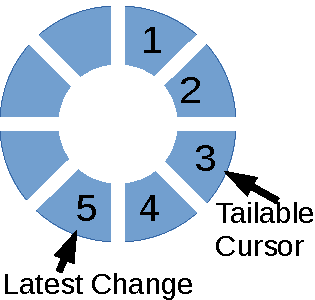
\includegraphics[width=0.3\textwidth]{draw/oplog-cursor}%
  \caption[Tailable cursor on the Oplog]{Tailable cursor on the Oplog}
  \vspace{-4mm}
  \label{fig:oplog-cursor}
\end{wrapfigure}
\reflst{lst:Oplog} shows an example document contained in the
Oplog. Besides the collection name and timestamp of the change, it
shows the type the causing operation (\texttt{op:"i"} stands for
insertion) and the inserted, updated, or removed document as
sub-document under the \texttt{o} key. For each new trigger, the
trigger manager creates a cursor on Oplog in MongoDB with the trigger
query. Initially this cursor points to the end of the Oplog (position
3 in \reffig{fig:oplog-cursor}). Because the Oplog is a capped
collection, new changes, e.g., 4 and 5 in \reffig{fig:oplog-cursor},
are appended behind the position the cursor points to. During the main
loop of Fawkes, the trigger manager checks for all tailable cursors if
there are new documents in the Oplog containing \texttt{o} object that match the according
query. As Oplog changes are checked, the tailable cursor is forwarded. Thus if
\reffig{lst:Oplog} shows the document labeled with 4 or 5 it would be
returned by the query.
The trigger manager then calls the callback function and passes the
document from \reffig{lst:Oplog}. This way, the application is
notified and can react to the change with the information contained in
the returned document from the Oplog.

\subsection{Unit-tests}
\label{sec:impl-unittests}
To ensure the quality and correctness of the robot memory, we
implemented unit tests for the important features of this layer. Unit
testing is part of the software development processes test driven
development and extreme programming~\cite{beck-test,beck-xp}. Unit
tests are automated software tests for small units of a program. They
use the functions or components that should be tested and check if the
computed result matches the expected one. Thus they help to locate
bugs, ensure the quality of the unit, and fasten the development
because they can verify if the tests still pass after changes in the
unit. We use unit tests for the robot memory by using the C++
interface of the robot memory and checking if the results are correct
for examples of common use cases. For example there is one test that
checks insert, update, and query operations by inserting a document
into an empty collection, updating it, and querying it by an updated
value. Another test checks if computables work by registering the
computable showed in \reflst{lst:comp-func} and \reflst{lst:comp},
executing the query in \reflst{lst:comp}b and checking if the result
matches \reflst{lst:comp}c. Unit-testing in Fawkes is based on Google's
C++ testing framework \emph{gtest}\footnote{\url{https://github.com/google/googletest}}. To test the functionality of the
robot memory in a fully running Fawkes process with dependencies of
the robot memory, such as the \texttt{mongodb} plugin, we integrated
our unit tests into a separate plugin that is started with the robot
memory when the tests are executed.
\todo[inline]{example unit-test}

\section{Application Interface}
\label{sec:impl-planner}
The application interface layer provides the features of the robot
memory for applications such as planners and reasoners. Components
written in C++ can directly interface the robot memory layer.
This interface is identical to the interface between the
robot memory and and the interface providers. For example perception
plugins in Fawkes are usually written in C++ and thus can provide
computables or store documents directly in the robot memory. Planner
and reasoner components often utilize specialized languages. For these
components and languages, there are multiple interface providers we
implemented. In the following, we present the interface providers for
PDDL, CLIPS, and OpenRAVE.

\subsection{PDDL Interface Provider}
\label{sec:impl-pddl}
To find a plan with a PDDL-based planner, a domain description and a problem
description need to be provided for the planner. The domain description
is usually fixed because the predicates defining the world state and
the actions defining the capabilities of the robot often are fixed for
a domain. The problem description, depends on the world model of the
robot and varies in the concrete predicates and the amount of
objects. Thus the problem description depends on the content of the
robot memory and has to be constructed before planning. This process
belongs to the model generation of the interface provider and is implemented in the
\texttt{pddl-robot-memory} plugin. In \refsec{sec:formalism}, we
defined the mapping from documents in the robot memory
to PDDL theoretically. Nevertheless, we need to specify which documents in the robot
memory should be mapped to PDDL and which strings are mapped to which
predicates, functions, and their attributes. These are the $name$
functions. To specify both, we make use of the template engine
\emph{ctemplate}\footnote{\url{https://code.google.com/p/google-ctemplate}}.
The template engine takes a \emph{template file} as
input and uses a \emph{dictionary} defined during run-time to exchange
\emph{template markers} in the file by desired string values.
\begin{figure}
  \begin{minipage}{0.58\linewidth}
\begin{lstlisting}[style=SmallPDDL,
  caption={PDDL problem description template},
  label=lst:template,
  framexleftmargin=1pt, xleftmargin=1pt,
 morekeywords={}, numbers=none]
(define (problem blocks_world_generated)
  (:domain blocksworld)
  (:objects A B C D)
  (:goal <<GOAL>>)
  (:init
    <<#ONTABLE|{relation:'on-table'}>>
      (on-table <<object>>) <</ONTABLE>>
    <<#ON|{relation:'on'}>>
      (on <<object_top>> <<object_bottom>>)
    <</ON>>
    <<#HOLDING|{relation:'holding'}>>
      (holding <<object>>) <</HOLDING>>
  ))
\end{lstlisting}
  \end{minipage}
\hfill
  \begin{minipage}{0.42\linewidth}
\begin{lstlisting}[style=SmallPDDL,
  caption={Generated PDDL problem description},
  label=lst:pddl-gen,
  framexleftmargin=1pt, xleftmargin=1pt,
 morekeywords={}, numbers=none]
(define (problem blocks_world_generated)
  (:domain blocksworld)
  (:objects A B C D)
  (:goal (on A B))
  (:init
    (on-table A)
    (on-table C)
    (on D A)
    (holding B)
  ))
\end{lstlisting}
\vspace{0.3cm}
  \end{minipage}
  \vspace{-0.8cm}
\end{figure}
An example template file for the blocks world domain is shown in
\reflst{lst:template}. The result after generating the problem
description based on information in the robot memory is shown in
\reflst{lst:pddl-gen}. A simple template marker is
\texttt{<<GOAL>>}. During the model generation, the dictionary is
filled with the information that \texttt{<<GOAL>>} should be replaced
by \texttt{(on A B)}. There also are special markers such as
\texttt{<<#ON>> <</ON>>}. They enclose an environment and are called
\emph{list markers} because they insert the enclosed environment for
each list entry of the dictionary on the \texttt{ON} marker. We use
list markers to insert a predicate for each document that is returned
by a query. The query is located in the front marker behind the
\texttt{|} symbol. The enclosed environment can contain markers that
are substituted by key-value pairs of documents. In the example given
in \reflst{lst:template}, the query \texttt{\{relation:'on-table'\}}
yields the documents \texttt{\{relation:'on-table', object:'A'\}},
what is mapped to \texttt{(on-table A)}, and
\texttt{\{relation:'on-table', object:'B'\}}, what is mapped to
\texttt{(on-table B)}. To distinguish markers inside these
environments, they are written in lower case.

The process of the model generation starts with an interface message
containing the goal to the \texttt{pddl-robot-memory} plugin. Then the
plugin parses the problem description template to extract the queries
of the list markers. This is a separate step, because passing
parameters to a list marker is not supported by ctemplate. The plugin
fills the dictionary with the goal and entries for each document
returned by the robot memory for a list marker query. For each such
list entry, all key-value pairs of the documents are inserted into the
dictionary, where the key name in the document equals the marker name
in the template. For sub-documents, the key names are concatenated so
that the marker name is the path to each value. Markers that are not
in the dictionary are later substituted by the empty string. Finally,
the dictionary is passed with the template file to ctemplate, which
generates the resulting problem description.

%mention problem that this template method can not recursively map
%function terms?

The direction from PDDL to the robot memory is implemented in the
\texttt{pddl-planner} plugin. When the plugin receives an interface
message, it starts the FF planner with the domain and generated
problem description files and waits until the planner finished. Then
the resulting plan is passed, transformed to a document as specified
in the theoretical foundation in \refsec{sec:formalism}, and inserted
into the robot memory. Afterwards an executive can fetch the plan, for
example after being notified by a trigger that there is a new plan.

\subsection{CLIPS Interface Provider}
\label{sec:impl-clips}
The Interface Provider for CLIPS is implemented in the
\texttt{clips-robot-memory} plugin as a CLIPS-feature. \emph{CLIPS-features} are extensions
of an environment, can be loaded during run-time, and can provide
access to C++ functions. In contrast to PDDL, CLIPS can use procedures. Thus
the CLIPS \emph{robot-memory feature} can wrap the interface functions
of the robot memory and provide them as functions inside the CLIPS
environment.
\begin{figure}
  \begin{lstlisting}[showlines,style=ReallySmallCLIPS, caption={CLIPS function to execute a query},
  label=lst:clips-rm,
  emph={skill, args, state, target, res},
  emphstyle=\bfseries\color{green!80!black},
  emph={[2]\?skill, \$\?args, wait-for-lock, \?target, use,
  WAIT-FOR-LOCK, SKILL-EXECUTION, running},
  emphstyle={[2]\bfseries\color{blue!80!black}},
  morekeywords={retract, assert, modify, skill-call, skill-to-execute,
    wait-for-lock}]
(rm-query "syncedrobmem.clipswm"
          (str-cat "{relation:'order', end:{$gt:" ?gametime "}}"))
\end{lstlisting} %$ This is just to fix Emacs highlighting due to dollar sign in code above
\end{figure}
\reflst{lst:clips-rm} shows an example function in CLIPS for querying
the robot memory. The function takes the collection name and the query
as a string concatenated by clips and yields a cursor to documents
about not ended orders. This cursor can then be used by further
functions to check if there are more documents, fetching the document,
and reading values from it. Furthermore, the robot-memory feature
provides higher abstracted functions, which can convert a fact
reference to a document and asserts facts constructed from
documents. These functions use a similar mapping as presented in the
theoretical foundation. The \texttt{relation} key-value pair is
matched to the fact template name and the other key-value pairs are
matched to slot names of this template. There is a transformation
between lists in CLIPS and sub-documents with numbered key-value
pairs. Other sub-documents are passed as reference to the
sub-document. 
\todo[inline]{example mapping doc-fact}

Similar to the model generation in PDDL, it is also possible to create
an initial fact base in CLIPS. This is done by querying the initial
state from the robot memory and asserting the corresponding facts to
the fact base. The robot-memory feature also provides access to
triggers, which are a good way to keep the fact base in CLIPS updated
according to changes in the robot memory. However, executing callback
functions to notify about triggers does not fit to the programming
methodology of the production system CLIPS. Rather CLIPS reacts to
events by having rules with facts representing the event in the
antecedent. Thus, when the CLIPS interface provider is notified about
a trigger activation, it asserts a fact representing this to the fact
base. This fact contains an identifier defined during the registration
of the trigger by a CLIPS agent, and a pointer to the Oplog document
causing the trigger event.

\subsection{OpenRAVE Interface Provider}
\label{sec:impl-openrave}
OpenRAVE is a motion planner that finds collision free paths and
movements of a robot, e.g., for an arm. It searches for the path in an
internal representation of the robot's environment, the
\emph{scene}. During setup or run-time, this scene is filled with
objects the robot knows about in its environment, either for
interaction or collision avoidance. To make sure the motion
planner scene is be consistent with the world model stored in the
robot memory, we implement the OpenRAVE interface provider in the
\texttt{openrave-robot-memory} plugin. The plugin constructs and
updates the motion planner scene from documents in the robot
memory. Based on configuration values, it queries the robot memory for
objects in the environment and inserts, updates, or removes them from
the OpenRAVE scene.
\begin{wrapfigure}{r}{0.35\textwidth}{6cm}
  \vspace{-0.8cm}
\begin{lstlisting}[style=SmallJSON,
  caption={Document used to construct the OpenRAVE scene},
  label=lst:openrave,
  framexleftmargin=5pt, xleftmargin=0pt,
 morekeywords={}, numbers=none]
{
  block: "B",
  frame: "map",
  translation:
   [0.43, -0.04, 0.01],
  rotation:
   [0, 0, 0.99, 0.08]
}
\end{lstlisting}
\vspace{-8mm}
\end{wrapfigure}
\reflst{lst:openrave} shows an example document, which can be used to
construct the OpenRAVE scene. The key-value pair \texttt{block:"B"}
specifies the type of the object and the name used to move or remove
it later. The type also defines the model used in the scene according
to the configuration. Furthermore the translation and rotation in a
given frame are used to place the object at the right position. Here,
the transform computable can be used to transform the position into
the frame used by OpenRAVE. For example the frame used for the Jaco
arm has its origin in the base of the arm.

\section{Application Scenarios}
\label{sec:applicationscenarios}
The two scenarios are chosen in a way that they
cover all major features of the robot memory and that they are
prototypes for applications the robot memory is made for.
In \refsec{sec:app-rcll}, we present how the robot memory is used in
the RCLL to synchronize the world model between multiple robots, and in
\refsec{sec:app-blocks-world}, we present the use of the robot memory
in a block stacking scenario with a robot arm.

\subsection{RoboCup Logistics League}
\label{sec:app-rcll}
A central component of
the Carologistics robot software in the RCLL is the CLIPS agent. It
maintains a world model, decides what the robot should do with
incremental reasoning~\cite{CLIPS-Agent}, and monitors the execution
of robot actions. The decision approach and world model maintenance is
distributed. Robots have to coordinate with each other and notify each
other about changes in the environment. Furthermore, they can drop out
and might be restarted. Thus, the CLIPS agent needs to synchronize its
world model with the other robots. The existing implementation used by
Carologistics in 2016 uses Protobuf messages which are being sent
between the agents. In this application scenario, we exchange the
synchronization via Protobuf by using the robot memory. Thus the world
model of CLIPS has to be represented in the robot memory and
distributed over all robots. On the one hand, this lays the foundation
for using the robot memory in the RCLL in future work. On the other
hand, this simplifies the CLIPS agent by separating the
synchronization. The synchronization by MongoDB is advantageous
because it only sends necessary changes over the network instead of
the whole world model, as it is done by the CLIPS agent. Another
advantage is the persistency, because robots keep their state if one
or even all of them are restarted.

\begin{figure}
  \centering
  \begin{subfigure}[b]{0.49\textwidth}
    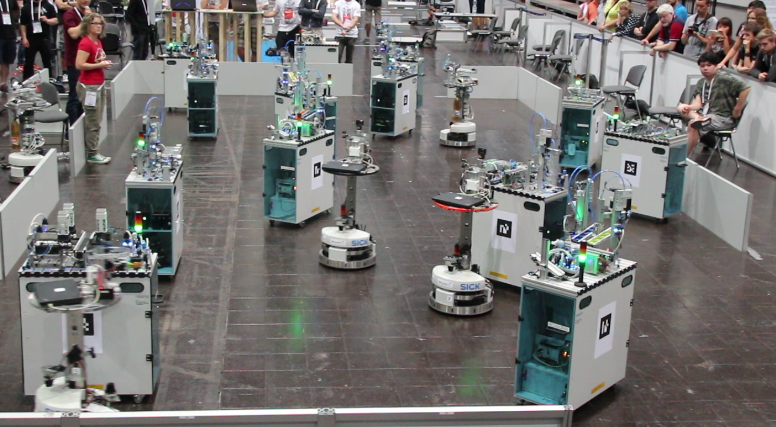
\includegraphics[width=\textwidth]{img/rcll-field}
    \caption{At the RoboCup 2016 in Leipzig}
    \label{fig:rcll-real}
  \end{subfigure}
\hfill
  \begin{subfigure}[b]{0.49\textwidth}
    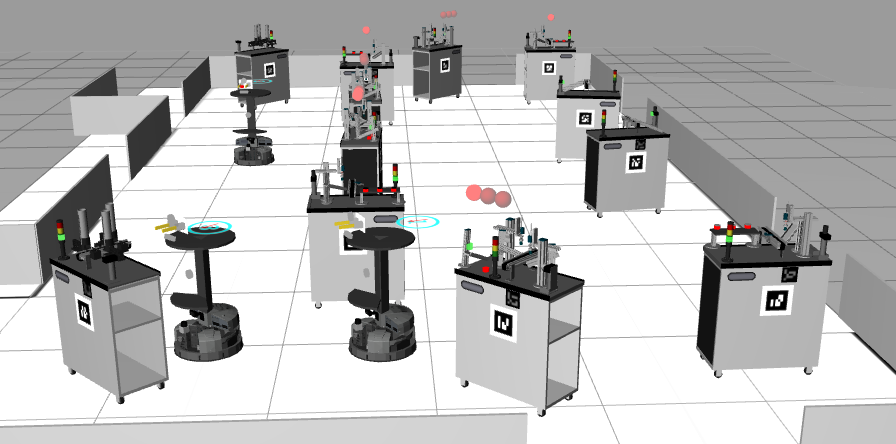
\includegraphics[width=\textwidth,height=0.55\textwidth]{img/rcll-sim}
    \caption{In the Gazebo simulation}
    \label{fig:rcll-sim}
  \end{subfigure}
  \caption[Field of the RoboCup Logistics League]{Field of the RoboCup Logistics League}
  \label{fig:rcll}
\end{figure}
During the development and evaluation of the RCLL scenario, we mainly
depend on the simulation of the RCLL shown in
\reffig{fig:rcll-sim}. This simplifies and fastens the development
because we had no full RCLL field available and properly setting up
all robots takes a lot effort. However, this does not make a
significant difference for the robot memory because the simulation can
be distributed over multiple machines and because the interface and
usage is identical in simulation and real world. Also the robot
behavior, perception results, and factory layout (\reffig{fig:rcll})
are similar. The environment agency by the Refbox is
identical. Different are WiFi issues occurring at RoboCup
competitions because the simulation only introduces a message loss for
UDP packages.

The distribution of the robot memory in the RCLL is achieved by
configuring the robot memory to use the replica set with all robots
and loading the \texttt{robot-memory} plugin on all robots of the
team. The world model existing in CLIPS is already properly
initialized at the start of the game and has to be transferred to the
robot memory. During the setup phase, one of the agents removes the
old world model in the robot memory, which persisted from a previous
game. Then all facts defining the world model are inserted into the
robot memory by using the fact-to-document function of the CLIPS
robot-memory feature. All facts that are represented in the robot
memory have the unique field \texttt{sync-id}. This field is used to
clearly identify which fact is represented by which document and vice
versa. During the game, facts inside CLIPS are modified, for example
because a robot commits to a task, observes a change, or applies the
effect of actions it performed. For this modification, the agent uses
the special modify function \texttt{(synced-modify)}, which uses a
syntax similar to the original \texttt{(modify)} function of
CLIPS. \texttt{(synced-modify)} applies the modification to the fact
that should be modified by calling \texttt{(modify)} and furthermore
updated the corresponding document in the robot memory by using the
\texttt{sync-id} in the query. Similarly there are the functions
\texttt{(synced-assert)} and \texttt{(synced-retract)}. Other robots
are notified about such a change in the robot memory by using
triggers. Each agent registers a trigger at its own
\texttt{robot-memory} plugin. Whenever there is a change, a trigger
fact is asserted according to \refsec{sec:impl-clips} and an update
rules consumes this fact and updates the fact with the corresponding
\texttt{sync-id}.

\subsection{Blocks World with a Robotic Arm}
\label{sec:app-blocks-world}
The second application scenario is the blocks world with a robotic
arm. Blocks world is a classical planning problem about planning the
actions of a robotic arm to stack blocks until a given goal state is
reached~\cite{blocks-world}. An example goal is stacking the blocks \texttt{A} on
\texttt{B} and \texttt{B} on \texttt{C}. If the initial state is shown
in \reffig{fig:blocksworld}, the planner has to figure out that a solving sequence of
actions is to put \texttt{A} on the table first, stack \texttt{B} on
\texttt{C} second, and stack \texttt{A} on
\texttt{B} third because the arm can only hold one block at a time.
Implementing this scenario with a real robot arm, is a good evaluation
scenario for the robot memory, because in contrast to the theoretical
problem, multiple components (perception, planners, executive)
have to work together and there are additional problems such as
occlusion and geometric representation and manipulation.
\begin{wrapfigure}{r}{0.37\textwidth}
  \centering
  \vspace{-6mm}
  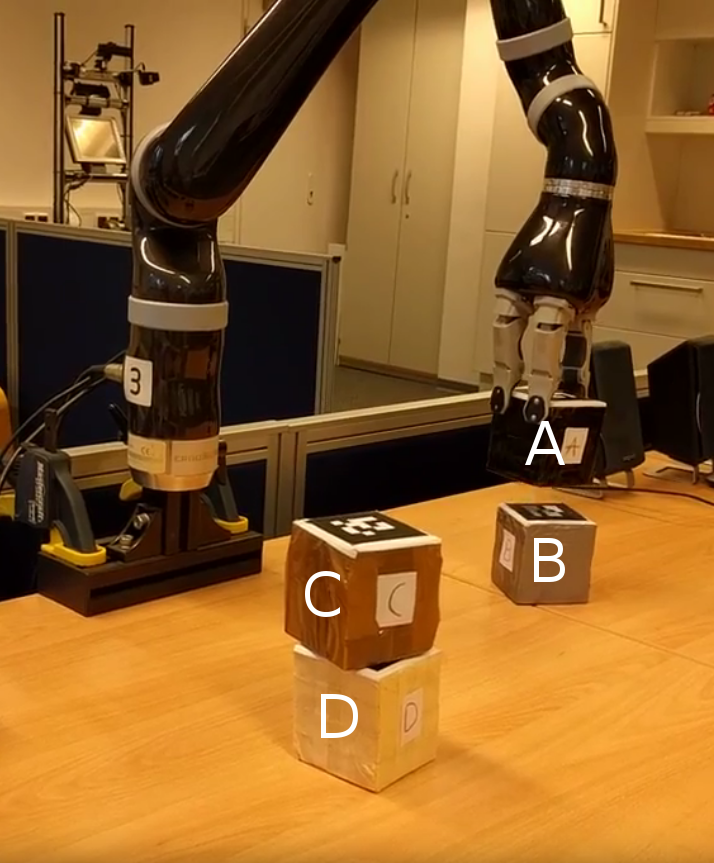
\includegraphics[width=0.37\textwidth]{img/blocks-world-annotated}%
  \caption[Blocks world scenario with Jaco arm (annotated)]{Blocks world scenario with Jaco arm (annotated)}
  \vspace{-4mm}
  \label{fig:blocksworld}
\end{wrapfigure}
\reffig{fig:blocksworld} shows this scenario and the Kinova Jaco arm
we are using. The scenario is inspired by the RoboCup@Home league,
which also deals with hybrid reasoning, perception, manipulation,
planning, and memorizing observations in the real world. Furthermore
we choose this scenario because it requires many features of
the robot memory. In the following, we present the different
components operating in this scenario and how they collaborate by
using the robot memory:
\\
\textbf{Perception:} Blocks are located and identified by a marker
attached to the top surface. We use the results of the detection by
the \texttt{tag-vision} plugin with a Kinect version 1 camera mounted
on the ceiling. We implemented the \texttt{blocks-world-perception}
plugin, which fetches the position of detected markers and updates the
last observed position in the robot memory. Because the
\texttt{tag-vision} plugin publishes its results on the blackboard, we
use the blackboard computable to obtain the interface data as
documents and the transform computable to transform block coordinates
from the camera frame into the map frame. Furthermore this plugin
provides computables for transforming the 3D positions into symbolic
information needed later by a PDDL component. It provides the symbolic
information if a block is on the table by comparing the height of the
block to the height of the table and if a block is clear to be grabbed
by checking if the marker is currently visible. There is also a
computable describing unknown blocks. If \reffig{fig:blocksworld}
shows the current situation, the plugin can detect that block
\texttt{C} is not on the table. By using the information in the robot
memory, the plugin also detects that there is an unknown block below
\texttt{C} because the robot memory does not contain any information
about \texttt{C} standing on another block yet.
\\
\textbf{PDDL-based planner:} The classical part of the blocks world scenario
is solved by a PDDL planner. There is a fixed domain description
describing the available predicates \texttt{on, holding, on-table,
  clear, arm-empty} and the possible arm actions \texttt{pickup,
  putdown, stack, unstack}. We use the PDDL robot memory interface to
generate the problem description based on the current state
represented in the robot memory. The template is an extended version
of \reflst{lst:template} and fills in the information, which is
memorized in the robot memory or provided by computables of the
\texttt{blocks-world-perception} plugin. All this information is
symbolic and spatial coordinates are filtered out so that the PDDL
planner can work with it. The resulting plan provided by the FF
planner is inserted into the robot memory.
\\
\textbf{CLIPS executive:} We use CLIPS executive as top level
executive for user interaction, invocation of the planner, and
monitoring plan execution. When a new goal state is specified by the
user, the executive invokes the PDDL model generation with the goal
first and then starts the planner. It uses a trigger to be notified
when the resulting plan is added to the robot memory. When planning
failed, it starts again, otherwise the plan is converted into a CLIPS
task with several steps as specified by the plan. The task-step
construction of the executive is also used in the RCLL CLIPS
agent. The task is executed step by step. For each step, the executive
calls the behavior engine~\cite{Behavior-Engine} to execute actions
defined in the step. Because the behavior engine requires the concrete
position where the arm should pick or put a block, the executive
queries the robot memory to obtain the position of the block with the
name given in the action. For the putdown action, the executive cycles
through free positions on the table. After successfully executing a
step, the executive updates the world model in the robot memory. For
example when block \texttt{B} was stacked on \texttt{C}, it adds a
document describing that \texttt{B} is now placed on \texttt{C} and
removes the document describing that \texttt{B} is hold. These updates
allow the system to remember the current state because the vision can
no longer detect \texttt{C} due to occlusion by \texttt{B}. When a
step fails, the execution of the plan is aborted and the executive
starts again with model generation and planning. In most cases, the
system can continue because the current state is remembered in the
robot memory.
\todo[inline]{listings clips (task+steps?)}
\\
\textbf{OpenRAVE motion planner:} The collision free motion of the arm
is planned with OpenRAVE.
\begin{wrapfigure}{r}{0.3\textwidth}
  \centering
  \vspace{-4mm}
  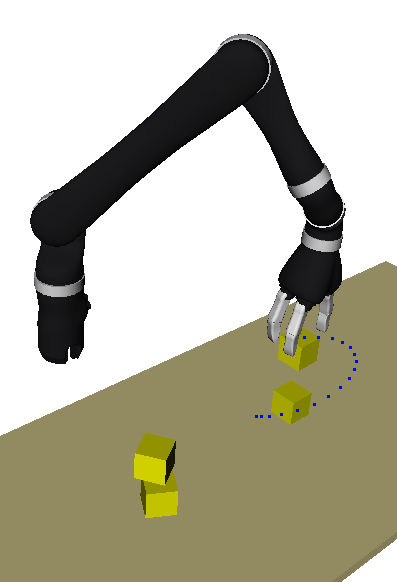
\includegraphics[width=0.3\textwidth]{img/openrave-blocks}%
  \caption[Blocks world OpenRAVE scene]{Blocks world OpenRAVE scene}
  \vspace{-4mm}
  \label{fig:openrave}
\end{wrapfigure}
\reffig{fig:openrave} shows the motion planner scene of OpenRAVE
and the path it planned in blue. The scene is constructed with by the OpenRAVE
robot memory interface, which queries the position, name, and type of
all objects in the environment from the robot memory. An example
document, which can be inserted from the robot memory into the
OpenRAVE scene is \reflst{lst:openrave}. Positions are
transformed by the transform computable into the frame of the robot
arm, which is used by OpenRAVE. The scene construction is invoked by
the executive between steps. The motion commands OpenRAVE plans and
controls are send by the behaviors executing each step.